\subsection[Neural Networks]{\textit{Neural Networks}}

%\subsubsection[Training e test set]{Training e test set}

%\begin{frame}
%
%	\frametitle{Neural Networks}
%
%	\begin{figure}[!htbp]
%		\centering
%		\includegraphics[width=0.90\linewidth]{images/supervised/z_algorithms_neural_networks/nn.jpeg}
%		%\caption{}
%	\end{figure}
%
%\end{frame}

\begin{frame}

	\frametitle{Neural Networks}

	\begin{figure}[!htbp]
		\centering
		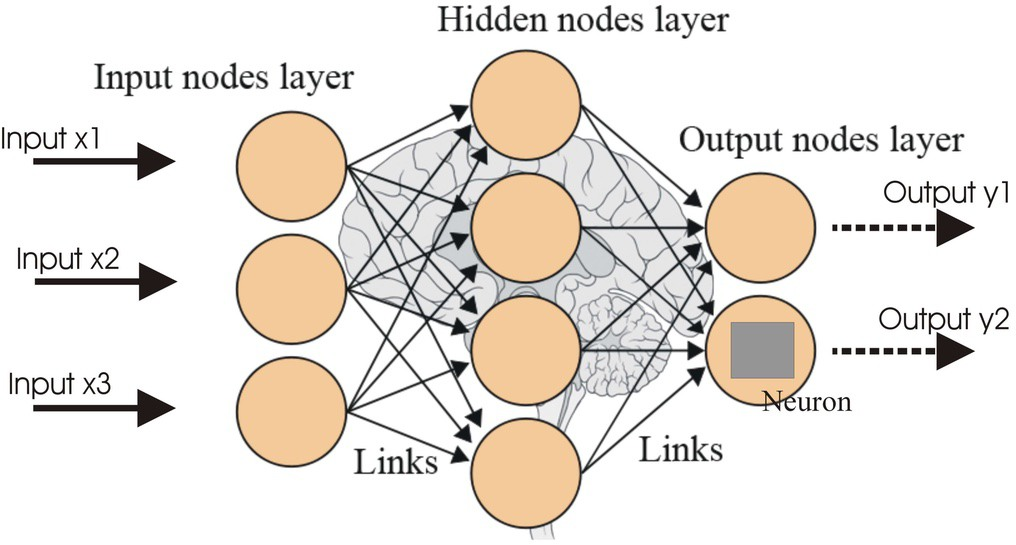
\includegraphics[width=1.00\linewidth]{images/supervised/z_algorithms_neural_networks/neural_network.jpg}
		%\caption{}
	\end{figure}

\end{frame}


\begin{frame}

	\frametitle{Neural Networks}

	Le reti neurali sono gli elementi costitutivi del progresso tecnologico di oggi nel campo del deep learning. Una rete neurale può essere vista come una semplice unità di elaborazione massicciamente parallela, in grado di immagazzinare conoscenza e applicarla per fare previsioni.
	\newlinedouble
	Una \textbf{rete neurale imita il cervello} nella modalità con il quale questa acquisisce conoscenza dal suo ambiente attraverso un processo di apprendimento.\\
	Quindi, le connessioni, noti come pesi sinaptici vengono utilizzati per memorizzare la conoscenza acquisita.\\
	Nel processo di apprendimento, i pesi sinaptici della rete vengono modificati in modo ordinato per raggiungere l'obiettivo desiderato.
	\newlinedouble
	Il \textbf{perceptron}, sviluppato da Rosenblatt nel 1958, è la rete neurale più semplice che separa linearmente i dati in due classi.

%	\begin{columns}
%		\column{0.8\linewidth}
%		Immaginiamo per un secondo di avere il problema di prevedere la probabilità di testa per alcuni lanci di moneta dove forse la moneta è leggermente piegata.
%
%		Potresti usare features come:
%		\begin{itemize}
%			\item angolo di piegatura
%			\item massa della moneta
%			\item o simili
%		\end{itemize}
%
%		\column{0.2\linewidth}
%		\begin{figure}[!htbp]
%			\centering
%			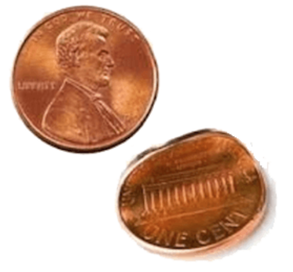
\includegraphics[width=1.0\linewidth]{images/supervised/z_algoritms_logistic_regression/flipped_coin.png}
%%			\caption{}
%		\end{figure}
%	\end{columns}
%	\ \\ 
%	Qual è il modello più semplice che potresti pensare di utilizzare?
%	\newlinedouble
%	Potremmo usare la regressione lineare.\\
%	Ma utilizzando tale modello potremmo avere degli strani risultati...\\
%	Ad esempio, cosa succede se abbiamo una nuova moneta che ha una massa molto pesante, che non abbiamo mai visto prima?\\
%	E cosa succede se abbiamo un angolo estremamente grande?
\end{frame}


\begin{frame}

	\frametitle{Neural Networks}

	\begin{figure}[!htbp]
		\centering
		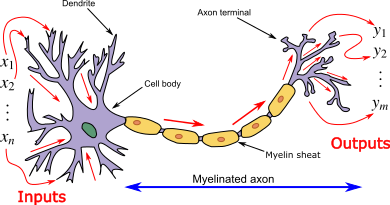
\includegraphics[width=0.90\linewidth]{images/supervised/z_algorithms_neural_networks/neuron.png}
		%\caption{}
	\end{figure}

\end{frame}


\begin{frame}

	\frametitle{Neural Networks}

	Il componente fondamentale delle reti neurali è il \textbf{neurone}, detto anche \textbf{unità neuronale} o semplicemente \textbf{unità}.\\
	\textbf{Molti neuroni}, sistemati in una struttura interconnessa, \textbf{vanno a formare una rete neurale}; ciascun neurone è collegato agli input e agli output degli altri. Un neurone può quindi ricevere input dagli esempi o dai risultati di altri neuroni, a seconda della sua posizione nella rete neurale.
	\begin{figure}[!htbp]
		\centering
		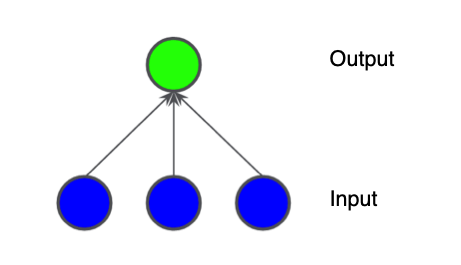
\includegraphics[width=0.45\linewidth]{images/supervised/z_algorithms_neural_networks/linear_net.png}
		\caption{Rappresentazione di un modello lineare sottoforma di rete neurale}
	\end{figure}
\end{frame}


\subsubsection[Single Layer Perceptron (SLP)]{Single Layer Perceptron (SLP)}
\begin{frame}

	\frametitle{Neural Networks: il perceptron (SLP)}

	Abbiamo visto qualcosa di simile al neurone, ossia il \textbf{perceptron}, il quale però utilizza una struttura e presenta un funzionamento più semplice.
	\newlinedouble
	Quando lo psicologo Rosenblatt concepì il perceptron, l'aveva pensato come a una \textbf{versione matematica semplificata di un neurone}.\\
	Un perceptron riceve in input dei valori dall'ambiente circostante (dataset), li pondera (in modo simile a come fanno le cellule cerebrali, in base alla forza delle connessioni all'interno dei legami stessi). Poi somma tutti i valori ponderati e si attiva quando la somma supera una determinata soglia.
	\newlinedouble
	Il perceptron, però, non è in grado di apprendere quando le classi che sta cercando di elaborare non sono separabili linearmente. Tuttavia anche se un singolo perceptron non può apprendere l'operazione logica XOR, la cosa diventa perfettamente fattibile nel momento in cui due percettroni lavorano insieme.
\end{frame}


\subsubsection[Multi Layer Perceptron (MLP)]{Multi Layer Perceptron (MLP)}
\begin{frame}

	\frametitle{Neural Networks: il multi-layer perceptron (MLP)}

	\begin{columns}
		\column{0.6\linewidth}
		Una versione più evoluta del SLP è il multi-layer perceptron, noto anche come \textbf{neural networks feed-forward} (letteralmente ``flusso in avanti''), è costituito da una sequenza di livelli, ciascuno completamente connesso a quello successivo.
		\newlinedouble
		Un \textbf{multi-layer perceptron (MLP)} ha uno o più livelli nascosti insieme ai livelli di input e output, ogni livello contiene diversi neuroni che si interconnettono tra loro tramite collegamenti pesati.

		\column{0.4\linewidth}
		\begin{figure}[!htbp]
			\centering
			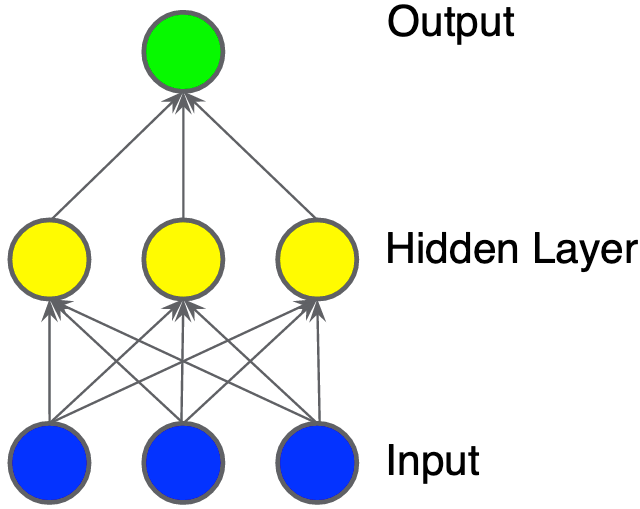
\includegraphics[width=1.0\linewidth]{images/supervised/z_algorithms_neural_networks/1hidden.png}
%			\caption{}
		\end{figure}
	\end{columns}
\end{frame}


\begin{frame}

	\frametitle{Neural Networks: il multi-layer perceptron (MLP)}

	\begin{columns}
		\column{0.6\linewidth}
		Il \textbf{numero di neuroni} nel livello \textbf{di input} sarà il \textbf{numero di attributi} del dataset, \textbf{i neuroni nel livello di output} rappresenterà il \textbf{numero di classi}.
		\newlinedouble
		Nel modello rappresentato dal grafico seguente, abbiamo aggiunto un ``livello nascosto'' di valori intermedi.
		\begin{itemize}
			\item ogni nodo giallo nel livello nascosto è una somma ponderata dei valori del nodo di input blu più un proprio bias
			\item l'output è una somma ponderata dei nodi gialli più quello specifico bias del nodo
		\end{itemize}

		\column{0.4\linewidth}
		\begin{figure}[!htbp]
			\centering
			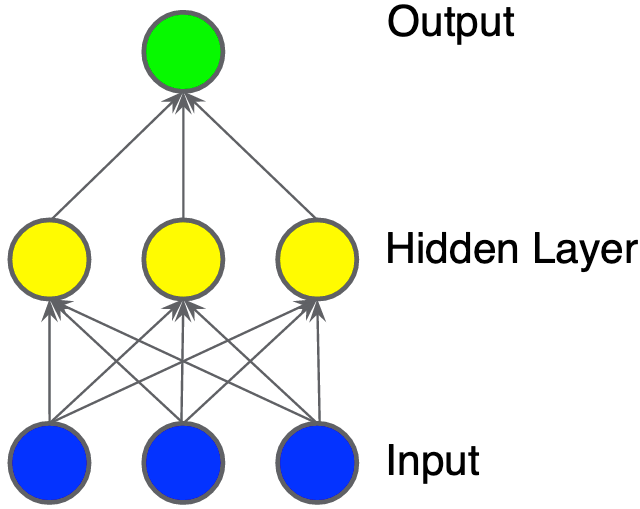
\includegraphics[width=1.0\linewidth]{images/supervised/z_algorithms_neural_networks/1hidden.png}
%			\caption{}
		\end{figure}
	\end{columns}

\end{frame}


\subsubsection[Gestire non-linearità]{Gestire non-linearità}
\begin{frame}

	\frametitle{Neural Networks: e se non linearmente separabili?}

	\begin{columns}
		\column{0.6\linewidth}
		Abbiamo appurato che abbiamo qualche \textbf{difficoltà in più} a modellare problemi non linearmente separabili.
		\newlinedouble
		Il primo esempio è stato lo \textbf{XOR}, anche se per questo caso specifico possiamo aggirare il problema utilizzando più modelli oppure introducendo delle \underline{\href{https://developers.google.com/machine-learning/crash-course/feature-crosses/encoding-nonlinearity}{feature crosses}}, tuttavia non è sempre così ``semplice''.
		\newlinedouble
		Un esempio potrebbe essere dato dalla \textbf{spirale non linearmente separabile} mostrata in figura.

		\column{0.4\linewidth}
		\begin{figure}[!htbp]
			\centering
			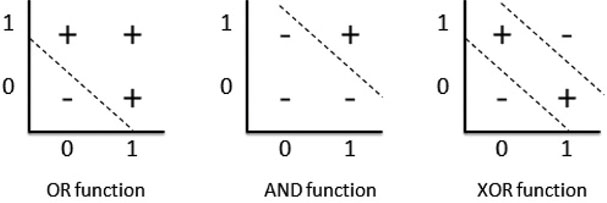
\includegraphics[width=1.0\linewidth]{images/supervised/z_algorithms_neural_networks/xor.jpg}
%			\caption{}
		\end{figure}
		\begin{figure}[!htbp]
			\centering
			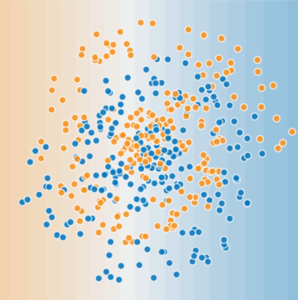
\includegraphics[width=0.7\linewidth]{images/supervised/z_algorithms_neural_networks/NonLinearSpiral.png}
%			\caption{}
		\end{figure}
	\end{columns}


\end{frame}


\begin{frame}

	\frametitle{Neural Networks: e se non linearmente separabili?}

	\begin{columns}
		\column{0.6\linewidth}
		Con le reti neurali viste fin qui, ogni livello nascosto in più introduce ``semplicemente'' una \textbf{combinazione lineare degli input del livello precedente}.
		\newlinedouble
		Quindi complessivamente i \textbf{modelli} con tale struttura, a prescindere dal numero di livelli nascosti introdotti, risultano comunque essere \textbf{lineari} perché una combinazione lineare di funzioni lineari è comunque lineare.

		\column{0.4\linewidth}
		\begin{figure}[!htbp]
			\centering
			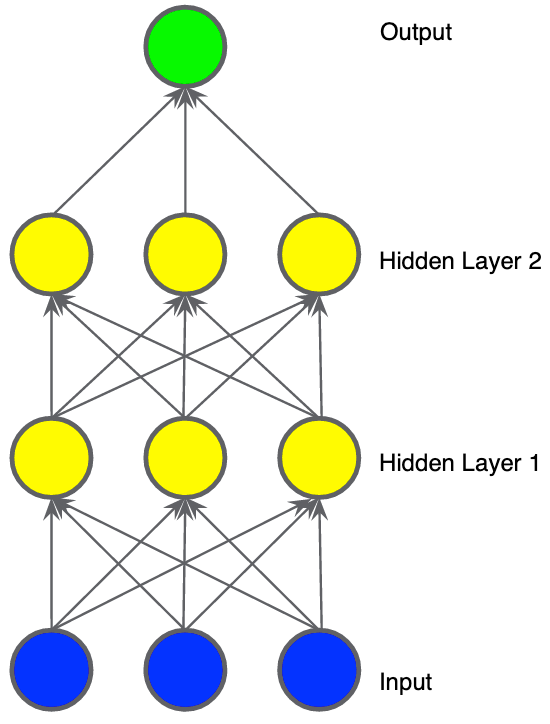
\includegraphics[width=1.0\linewidth]{images/supervised/z_algorithms_neural_networks/2hidden.png}
%			\caption{}
		\end{figure}
	\end{columns}


\end{frame}


\subsubsection[Funzioni di attivazione]{Funzioni di attivazione}

\begin{frame}

	\frametitle{Neural Networks: modelliamo delle non linearità}

	\begin{columns}
		\column{0.6\linewidth}
		Per modellare un problema non lineare, possiamo introdurre direttamente una non linearità. Possiamo far passare ogni nodo di un livello nascosto attraverso una funzione non lineare.
		\newlinedouble
		Nel modello rappresentato dal grafico seguente, il valore di ogni nodo in \textit{Hidden Layer 1} viene trasformato da una \textbf{funzione non lineare} prima di essere passato alle somme ponderate del layer successivo. Questa funzione non lineare è chiamata \textbf{funzione di attivazione}.\\
		\textit{Spesso le trasformazioni non lineari non sono rappresentate graficamente sottoforma di neuroni}.

		\column{0.4\linewidth}
		\begin{figure}[!htbp]
			\centering
			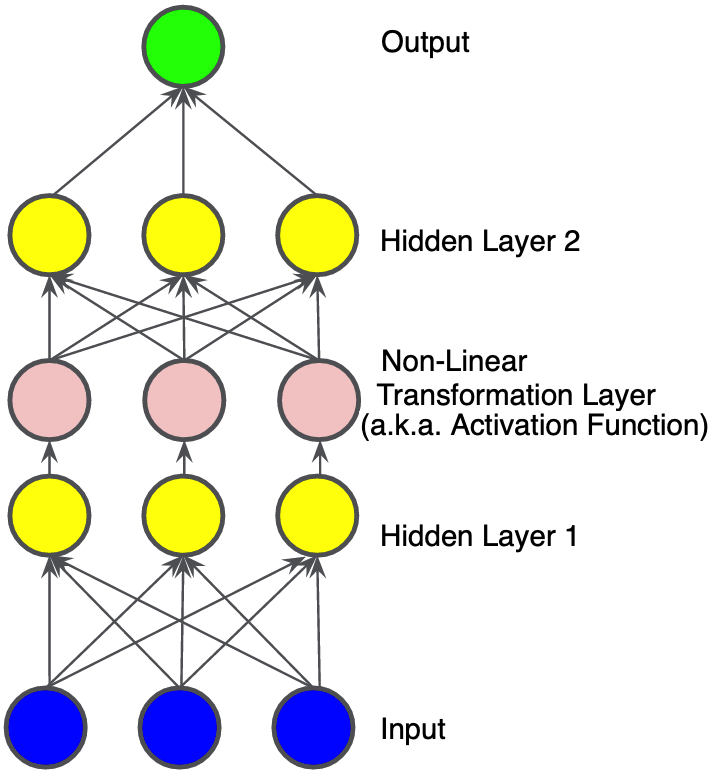
\includegraphics[width=1.05\linewidth]{images/supervised/z_algorithms_neural_networks/activation.png}
%			\caption{}
		\end{figure}
	\end{columns}


\end{frame}


\begin{frame}

	\frametitle{Neural Networks: alcune funzioni di attivazione}

	Ora che abbiamo aggiunto una \textbf{funzione di attivazione}, l'aggiunta di livelli ha un impatto maggiore. Impilare delle non linearità sulle non linearità ci consente di modellare \textbf{relazioni molto complicate} tra gli input e gli output previsti. In breve, ogni livello sta effettivamente apprendendo una funzione più complessa e di livello superiore a partire dagli input grezzi.

	\begin{columns}
		\column{0.6\linewidth}
		\begin{itemize}
			\item \textbf{Sigmoide}:\\
				converte una somma pesata in un valore tra 0 e 1
				$$g(z) = \frac{1}{1 + e^{-z}}$$
			\item \textbf{ReLu} (rectified linear unit):
				$$g(z) = max(0, z)$$
		\end{itemize}

		\column{0.4\linewidth}
		\begin{figure}[!htbp]
			\centering
			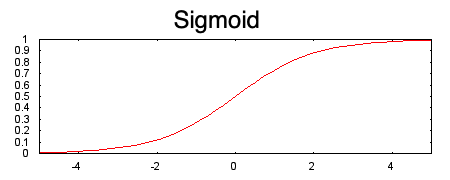
\includegraphics[width=1.0\linewidth]{images/supervised/z_algorithms_neural_networks/sigmoid.png}
%			\caption{}
		\end{figure}
		\begin{figure}[!htbp]
			\centering
			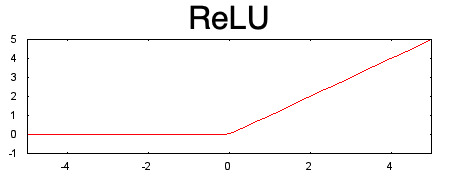
\includegraphics[width=1.0\linewidth]{images/supervised/z_algorithms_neural_networks/relu.png}
%			\caption{}
		\end{figure}
	\end{columns}


\end{frame}


\begin{frame}

	\frametitle{Neural Networks: funzioni di attivazione}

	In effetti, qualsiasi funzione matematica può servire come funzione di attivazione.
	\newlinedouble
	Supponiamo che $\sigma$ rappresenti la nostra funzione di attivazione.\\
	Il valore di un nodo nella rete è dato dalla seguente formula:

	\begin{itemize}
		\item $g(z) = \sigma(z) = \sigma(\pmb{w} \cdot \pmb{a}+\pmb{b})$
	\end{itemize}
	
	\begin{figure}[!htbp]
		\centering
		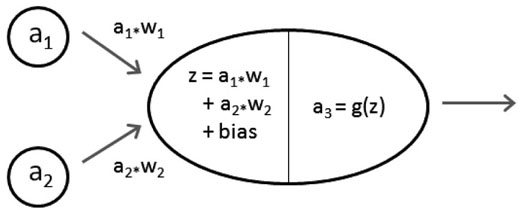
\includegraphics[width=0.5\linewidth]{images/supervised/z_algorithms_neural_networks/neuron.jpg}
		%\caption{}
	\end{figure}
	Al seguente \underline{\href{https://www.tensorflow.org/api_docs/python/tf/nn}{link}} puoi trovare una lista di quelle che sono le funzioni di attivazione disponibili in \underline{\href{https://www.tensorflow.org/}{TensorFlow}}.

	
\end{frame}


\begin{frame}

	\frametitle{Neural Networks: funzioni di attivazione}

	\begin{figure}[!htbp]
		\centering
		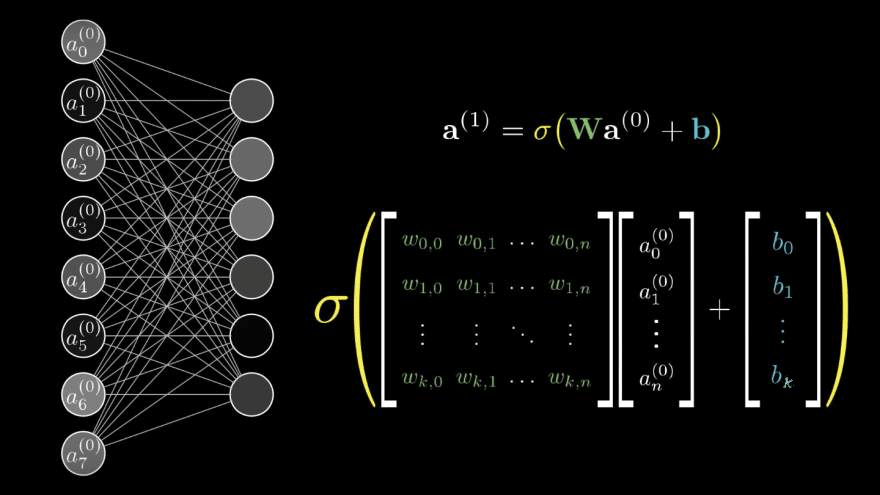
\includegraphics[width=1.0\linewidth]{images/supervised/z_algorithms_neural_networks/nn_sigma_formula.png}
		%\caption{}
	\end{figure}

\end{frame}



\subsubsection[OvA e Softmax]{OvA e Softmax}
\begin{frame}

	\frametitle{Neural Networks: OvA e Softmax}

	Due layers particolari per gestire gli output per problemi multiclasse sono:

	\begin{itemize}
		\item \textbf{One vs All}:\\
			dato un problema di classificazione con $N$ possibili soluzioni, la OvA consiste nel realizzare $N$ classificatori binari separati, un classificatore binario per ogni possibile risultato. Durante l'addestramento, il modello esegue una sequenza di classificatori binari, addestrando ciascuno a rispondere a una domanda di classificazione separata.
		\item \textbf{Softmax}: $p(y = j|\textbf{x})  = \frac{e^{(\textbf{w}_j^{T}\textbf{x} + b_j)}}{\sum_{k\in K} {e^{(\textbf{w}_k^{T}\textbf{x} + b_k)}} }$\\
			la regressione logistica produce un decimale compreso tra 0 e 1.0.\\
			Ad esempio, un output di regressione logistica di 0,8 per un classificatore di e-mail suggerisce una probabilità dell'80\% che un'e-mail sia spam (contro il 20\% che non lo sia).
			Softmax estende questa idea in un mondo multi-classe. Cioè, Softmax assegna probabilità decimali a ciascuna classe di un problema multi-classe (la cui somma complessiva farà 1.0).
	\end{itemize}

\end{frame}


\begin{frame}

	\frametitle{Neural Networks: OvA e Softmax}

	\begin{columns}
		\column{0.5\linewidth}
		\begin{figure}[!htbp]
			\centering
			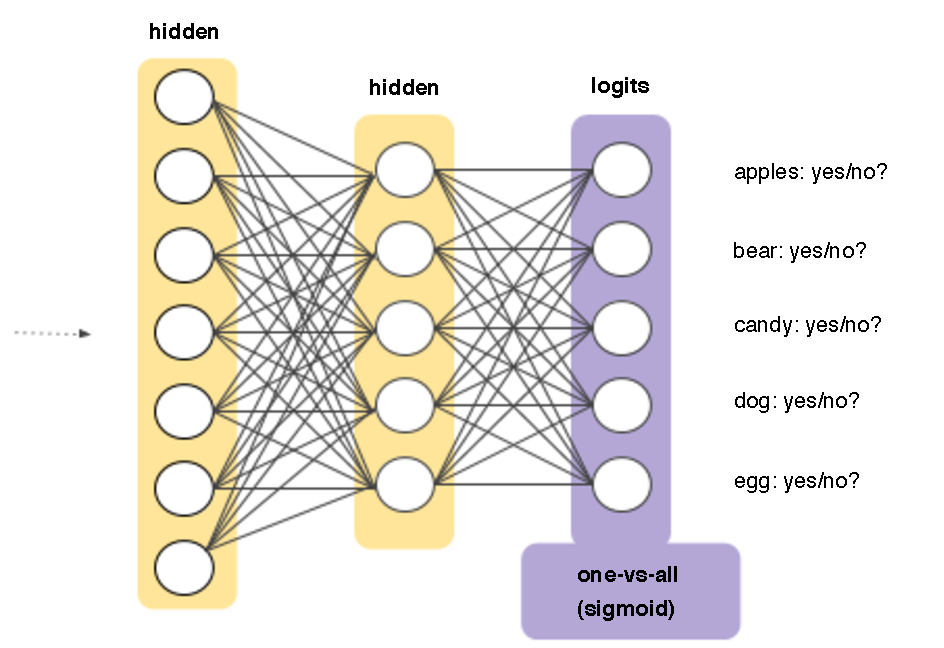
\includegraphics[width=1.0\linewidth]{images/supervised/z_algorithms_neural_networks/OneVsAll.pdf}
%			\caption{}
		\end{figure}

		\begin{scriptsize}
			\begin{table}[]
				\begin{tabular}{|c|c|}
				\hline
				\rowcolor{gray!50} \textbf{Class} & \textbf{Probability}\\ \hline
				apple & No\\ \hline
				bear & No\\ \hline
				candy & No\\ \hline
				dog & Yes\\ \hline
				egg & No\\ \hline
				\end{tabular}
			\end{table}
		\end{scriptsize}


		\column{0.5\linewidth}
		\begin{figure}[!htbp]
			\centering
			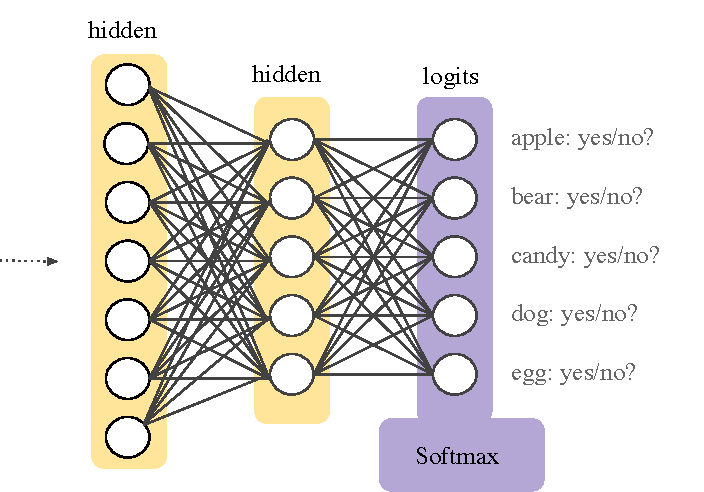
\includegraphics[width=1.0\linewidth]{images/supervised/z_algorithms_neural_networks/SoftmaxLayer.pdf}
%			\caption{}
		\end{figure}

		\begin{scriptsize}
			\begin{table}[]
				\begin{tabular}{|c|c|}
				\hline
				\rowcolor{gray!50} \textbf{Class} & \textbf{Probability}\\ \hline
				apple & 0.001\\ \hline
				bear & 0.04\\ \hline
				candy & 0.008\\ \hline
				dog & 0.95\\ \hline
				egg & 0.001\\ \hline
				\end{tabular}
			\end{table}
		\end{scriptsize}

	\end{columns}

\end{frame}


\subsubsection[Backpropagation]{Backpropagation}
\begin{frame}

	\frametitle{Backpropagation}

	Nella regressione lineare, è banale trovare una regola di aggiornamento per \textbf{modificare al meglio ciascun parametro} (il vettore dei coefficienti), mentre in una \textbf{rete neurale} le cose si fanno un pochino \textbf{più complicate}.
	\newlinedouble
	L'architettura è variabile e i coefficienti dei parametri (le connessioni) sono correlati fra loro perché le connessioni in un livello dipendono dal modo in cui le connessioni dei livelli precedenti hanno ricombinato gli input.
	\newlinedouble
	La soluzione a questo problema è l'algoritmo di \textbf{backpropagation}: si tratta di un modo intelligente per propagare all'indietro gli errori nella rete e fare in modo che ciascuna connessione modifichi di conseguenza i propri pesi. Se all'inizio si fanno avanzare sulla rete le informazioni propagate, bisogna tornare indietro e fornire il feedback su ciò che è andato storto mentre le informazioni scorrevano in quella direzione.
\end{frame}


\begin{frame}

	\frametitle{Neural Networks: un riepilogo}

	Ora il nostro modello ha tutti i componenti standard di ciò che le persone di solito intendono quando dicono \textbf{neural network}:
	\begin{itemize}
		\item un insieme di nodi, di neuroni, organizzati in strati
		\item un insieme di pesi che rappresentano le connessioni tra ogni livello della neural network e il livello sottostante
		\item un insieme di biases, uno per ogni nodo
		\item una funzione di attivazione che trasforma l'output di ogni nodo in uno strato. Livelli diversi possono avere funzioni di attivazione diverse
	\end{itemize}
	
%	\begin{columns}
%		\column{0.5\linewidth}
%		\begin{figure}[!htbp]
%			\centering
%			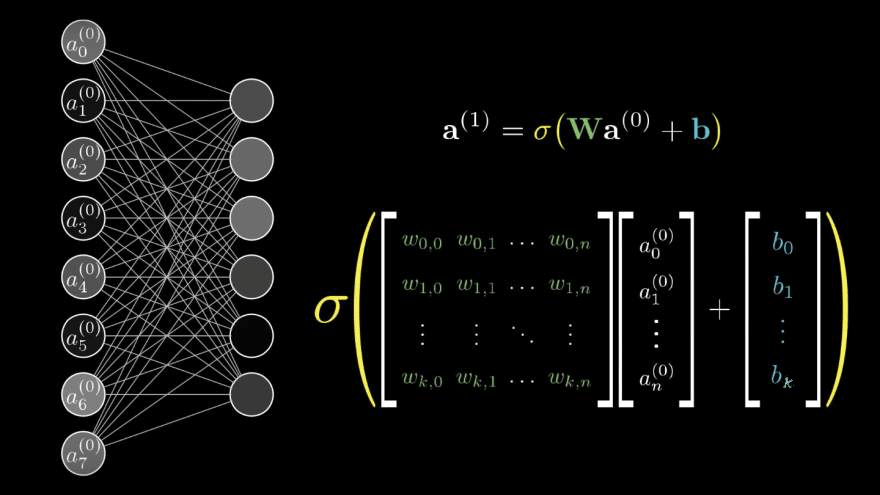
\includegraphics[width=1.0\linewidth]{images/supervised/z_algorithms_neural_networks/nn_sigma_formula.jpeg}
%			%\caption{}
%		\end{figure}
%
%
%		\column{0.5\linewidth}
%		\begin{figure}[!htbp]
%			\centering
%			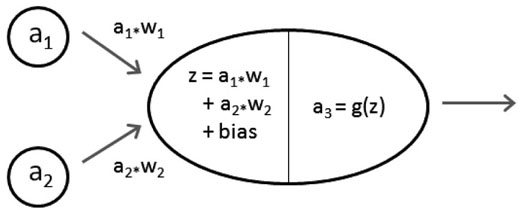
\includegraphics[width=1.0\linewidth]{images/supervised/z_algorithms_neural_networks/neuron.jpg}
%			%\caption{}
%		\end{figure}
%
%	\end{columns}

\end{frame}



% Le reti neurali, quando sono congegnate usando alcune specifiche tecnicità, prendono il nome di deep learning (letteralmente “apprendimento profondo”) e sono alla base di strumenti potenti come Siri e altri assistenti digitali, nonché di alcune delle più stupefacenti applicazioni di machine learning. Per esempio, le potete vedere al lavoro in questa incredibile dimostrazione di Rick Rashid, CEO di Microsoft, che parla in inglese mentre viene tradotto simultaneamente in cinese: https://www.youtube.com/watch?v=Nu-nlQqFCKg. Se il sogno dell'intelligenza artificiale si sta davvero per avverare, sembra assai probabile che siano proprio le reti neurali a realizzarlo.

% “Il principio è che i dati processati da una rete fluiscono sempre in avanti. Nelle reti classiche questo vuol dire passare allo strato neuronale successivo. Nel deep learning, di cui parleremo dopo, i dati da uno strato possono passare contemporaneamente anche a più strati neuronali successivi. Il passaggio avviene però sempre e comunque in avanti.
%Utilizzare una rete neurale è come utilizzare un sistema di filtraggio stratificato per l'acqua: l'acqua viene versata nella parte superiore, quindi esce filtrata dalla parte inferiore. Non può in alcun modo tornare indietro: prosegue in avanti e verso il basso, mai di lato. Analogamente, le reti neurali costringono le feature a fluire lungo la rete e a mescolarsi le une con le altre solo seguendo l'architettura della rete.
%Utilizzando l'architettura più adeguata a processare insieme le feature, la rete neurale riesce a creare nuove feature composite come risultato di ciascun livello in cui i dati fluiscono, il che porta alla fine ad avere previsioni migliori. Purtroppo, non esiste un modo per stabilire quale sia l'architettura migliore, se non provando empiricamente o sistematicamente soluzioni diverse e verificando se i dati in uscita come risultati prevedono i valori target dopo essere passati attraverso la rete.
